\documentclass[1p]{elsarticle_modified}
%\bibliographystyle{elsarticle-num}

%\usepackage[colorlinks]{hyperref}
%\usepackage{abbrmath_seonhwa} %\Abb, \Ascr, \Acal ,\Abf, \Afrak
\usepackage{amsfonts}
\usepackage{amssymb}
\usepackage{amsmath}
\usepackage{amsthm}
\usepackage{scalefnt}
\usepackage{amsbsy}
\usepackage{kotex}
\usepackage{caption}
\usepackage{subfig}
\usepackage{color}
\usepackage{graphicx}
\usepackage{xcolor} %% white, black, red, green, blue, cyan, magenta, yellow
\usepackage{float}
\usepackage{setspace}
\usepackage{hyperref}

\usepackage{tikz}
\usetikzlibrary{arrows}

\usepackage{multirow}
\usepackage{array} % fixed length table
\usepackage{hhline}

%%%%%%%%%%%%%%%%%%%%%
\makeatletter
\renewcommand*\env@matrix[1][\arraystretch]{%
	\edef\arraystretch{#1}%
	\hskip -\arraycolsep
	\let\@ifnextchar\new@ifnextchar
	\array{*\c@MaxMatrixCols c}}
\makeatother %https://tex.stackexchange.com/questions/14071/how-can-i-increase-the-line-spacing-in-a-matrix
%%%%%%%%%%%%%%%

\usepackage[normalem]{ulem}

\newcommand{\msout}[1]{\ifmmode\text{\sout{\ensuremath{#1}}}\else\sout{#1}\fi}
%SOURCE: \msout is \stkout macro in https://tex.stackexchange.com/questions/20609/strikeout-in-math-mode

\newcommand{\cancel}[1]{
	\ifmmode
	{\color{red}\msout{#1}}
	\else
	{\color{red}\sout{#1}}
	\fi
}

\newcommand{\add}[1]{
	{\color{blue}\uwave{#1}}
}

\newcommand{\replace}[2]{
	\ifmmode
	{\color{red}\msout{#1}}{\color{blue}\uwave{#2}}
	\else
	{\color{red}\sout{#1}}{\color{blue}\uwave{#2}}
	\fi
}

\newcommand{\Sol}{\mathcal{S}} %segment
\newcommand{\D}{D} %diagram
\newcommand{\A}{\mathcal{A}} %arc


%%%%%%%%%%%%%%%%%%%%%%%%%%%%%5 test

\def\sl{\operatorname{\textup{SL}}(2,\Cbb)}
\def\psl{\operatorname{\textup{PSL}}(2,\Cbb)}
\def\quan{\mkern 1mu \triangleright \mkern 1mu}

\theoremstyle{definition}
\newtheorem{thm}{Theorem}[section]
\newtheorem{prop}[thm]{Proposition}
\newtheorem{lem}[thm]{Lemma}
\newtheorem{ques}[thm]{Question}
\newtheorem{cor}[thm]{Corollary}
\newtheorem{defn}[thm]{Definition}
\newtheorem{exam}[thm]{Example}
\newtheorem{rmk}[thm]{Remark}
\newtheorem{alg}[thm]{Algorithm}

\newcommand{\I}{\sqrt{-1}}
\begin{document}

%\begin{frontmatter}
%
%\title{Boundary parabolic representations of knots up to 8 crossings}
%
%%% Group authors per affiliation:
%\author{Yunhi Cho} 
%\address{Department of Mathematics, University of Seoul, Seoul, Korea}
%\ead{yhcho@uos.ac.kr}
%
%
%\author{Seonhwa Kim} %\fnref{s_kim}}
%\address{Center for Geometry and Physics, Institute for Basic Science, Pohang, 37673, Korea}
%\ead{ryeona17@ibs.re.kr}
%
%\author{Hyuk Kim}
%\address{Department of Mathematical Sciences, Seoul National University, Seoul 08826, Korea}
%\ead{hyukkim@snu.ac.kr}
%
%\author{Seokbeom Yoon}
%\address{Department of Mathematical Sciences, Seoul National University, Seoul, 08826,  Korea}
%\ead{sbyoon15@snu.ac.kr}
%
%\begin{abstract}
%We find all boundary parabolic representation of knots up to 8 crossings.
%
%\end{abstract}
%\begin{keyword}
%    \MSC[2010] 57M25 
%\end{keyword}
%
%\end{frontmatter}

%\linenumbers
%\tableofcontents
%
\newcommand\colored[1]{\textcolor{white}{\rule[-0.35ex]{0.8em}{1.4ex}}\kern-0.8em\color{red} #1}%
%\newcommand\colored[1]{\textcolor{white}{ #1}\kern-2.17ex	\textcolor{white}{ #1}\kern-1.81ex	\textcolor{white}{ #1}\kern-2.15ex\color{red}#1	}

{\Large $\underline{12a_{0139}~(K12a_{0139})}$}

\setlength{\tabcolsep}{10pt}
\renewcommand{\arraystretch}{1.6}
\vspace{1cm}\begin{tabular}{m{100pt}>{\centering\arraybackslash}m{274pt}}
\multirow{5}{120pt}{
	\centering
	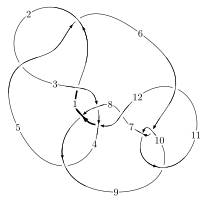
\includegraphics[width=112pt]{../../../GIT/diagram.site/Diagrams/png/940_12a_0139.png}\\
\ \ \ A knot diagram\footnotemark}&
\allowdisplaybreaks
\textbf{Linearized knot diagam} \\
\cline{2-2}
 &
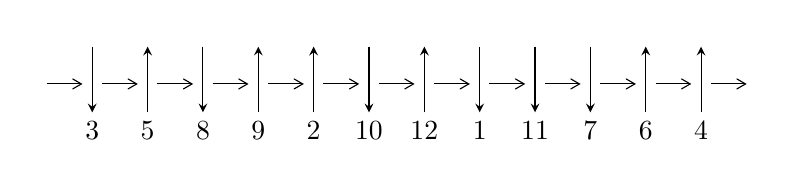
\begin{tikzpicture}[x=20pt, y=17pt]
	% nodes
	\node (C0) at (0, 0) {};
	\node (C1) at (1, 0) {};
	\node (C1U) at (1, +1) {};
	\node (C1D) at (1, -1) {3};

	\node (C2) at (2, 0) {};
	\node (C2U) at (2, +1) {};
	\node (C2D) at (2, -1) {5};

	\node (C3) at (3, 0) {};
	\node (C3U) at (3, +1) {};
	\node (C3D) at (3, -1) {8};

	\node (C4) at (4, 0) {};
	\node (C4U) at (4, +1) {};
	\node (C4D) at (4, -1) {9};

	\node (C5) at (5, 0) {};
	\node (C5U) at (5, +1) {};
	\node (C5D) at (5, -1) {2};

	\node (C6) at (6, 0) {};
	\node (C6U) at (6, +1) {};
	\node (C6D) at (6, -1) {10};

	\node (C7) at (7, 0) {};
	\node (C7U) at (7, +1) {};
	\node (C7D) at (7, -1) {12};

	\node (C8) at (8, 0) {};
	\node (C8U) at (8, +1) {};
	\node (C8D) at (8, -1) {1};

	\node (C9) at (9, 0) {};
	\node (C9U) at (9, +1) {};
	\node (C9D) at (9, -1) {11};

	\node (C10) at (10, 0) {};
	\node (C10U) at (10, +1) {};
	\node (C10D) at (10, -1) {7};

	\node (C11) at (11, 0) {};
	\node (C11U) at (11, +1) {};
	\node (C11D) at (11, -1) {6};

	\node (C12) at (12, 0) {};
	\node (C12U) at (12, +1) {};
	\node (C12D) at (12, -1) {4};
	\node (C13) at (13, 0) {};

	% arrows
	\draw[->,>={angle 60}]
	(C0) edge (C1) (C1) edge (C2) (C2) edge (C3) (C3) edge (C4) (C4) edge (C5) (C5) edge (C6) (C6) edge (C7) (C7) edge (C8) (C8) edge (C9) (C9) edge (C10) (C10) edge (C11) (C11) edge (C12) (C12) edge (C13) ;	\draw[->,>=stealth]
	(C1U) edge (C1D) (C2D) edge (C2U) (C3U) edge (C3D) (C4D) edge (C4U) (C5D) edge (C5U) (C6U) edge (C6D) (C7D) edge (C7U) (C8U) edge (C8D) (C9U) edge (C9D) (C10U) edge (C10D) (C11D) edge (C11U) (C12D) edge (C12U) ;
	\end{tikzpicture} \\
\hhline{~~} \\& 
\textbf{Solving Sequence} \\ \cline{2-2} 
 &
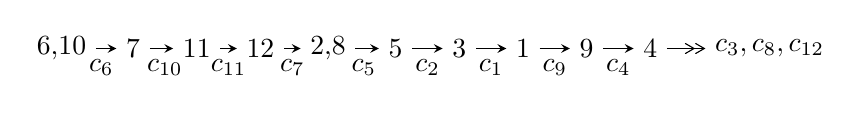
\begin{tikzpicture}[x=23pt, y=7pt]
	% node
	\node (A0) at (-1/8, 0) {6,10};
	\node (A1) at (1, 0) {7};
	\node (A2) at (2, 0) {11};
	\node (A3) at (3, 0) {12};
	\node (A4) at (65/16, 0) {2,8};
	\node (A5) at (41/8, 0) {5};
	\node (A6) at (49/8, 0) {3};
	\node (A7) at (57/8, 0) {1};
	\node (A8) at (65/8, 0) {9};
	\node (A9) at (73/8, 0) {4};
	\node (C1) at (1/2, -1) {$c_{6}$};
	\node (C2) at (3/2, -1) {$c_{10}$};
	\node (C3) at (5/2, -1) {$c_{11}$};
	\node (C4) at (7/2, -1) {$c_{7}$};
	\node (C5) at (37/8, -1) {$c_{5}$};
	\node (C6) at (45/8, -1) {$c_{2}$};
	\node (C7) at (53/8, -1) {$c_{1}$};
	\node (C8) at (61/8, -1) {$c_{9}$};
	\node (C9) at (69/8, -1) {$c_{4}$};
	\node (A10) at (11, 0) {$c_{3},c_{8},c_{12}$};

	% edge
	\draw[->,>=stealth]	
	(A0) edge (A1) (A1) edge (A2) (A2) edge (A3) (A3) edge (A4) (A4) edge (A5) (A5) edge (A6) (A6) edge (A7) (A7) edge (A8) (A8) edge (A9) ;
	\draw[->>,>={angle 60}]	
	(A9) edge (A10);
\end{tikzpicture} \\ 

\end{tabular} \\

\footnotetext{
The image of knot diagram is generated by the software ``\textbf{Draw programme}" developed by Andrew Bartholomew(\url{http://www.layer8.co.uk/maths/draw/index.htm\#Running-draw}), where we modified some parts for our purpose(\url{https://github.com/CATsTAILs/LinksPainter}).
}\phantom \\ \newline 
\centering \textbf{Ideals for irreducible components\footnotemark of $X_{\text{par}}$} 
 
\begin{align*}
I^u_{1}&=\langle 
-1.34404\times10^{85} u^{129}-2.83677\times10^{85} u^{128}+\cdots+3.31526\times10^{84} b-1.05008\times10^{85},\\
\phantom{I^u_{1}}&\phantom{= \langle  }1.17862\times10^{85} u^{129}+2.09114\times10^{85} u^{128}+\cdots+3.31526\times10^{84} a+7.72033\times10^{84},\;u^{130}+3 u^{129}+\cdots-2 u+1\rangle \\
I^u_{2}&=\langle 
b- a-1,\;a^2+a+1,\;u-1\rangle \\
\\
\end{align*}
\raggedright * 2 irreducible components of $\dim_{\mathbb{C}}=0$, with total 132 representations.\\
\footnotetext{All coefficients of polynomials are rational numbers. But the coefficients are sometimes approximated in decimal forms when there is not enough margin.}
\newpage
\renewcommand{\arraystretch}{1}
\centering \section*{I. $I^u_{1}= \langle -1.34\times10^{85} u^{129}-2.84\times10^{85} u^{128}+\cdots+3.32\times10^{84} b-1.05\times10^{85},\;1.18\times10^{85} u^{129}+2.09\times10^{85} u^{128}+\cdots+3.32\times10^{84} a+7.72\times10^{84},\;u^{130}+3 u^{129}+\cdots-2 u+1 \rangle$}
\flushleft \textbf{(i) Arc colorings}\\
\begin{tabular}{m{7pt} m{180pt} m{7pt} m{180pt} }
\flushright $a_{6}=$&$\begin{pmatrix}1\\0\end{pmatrix}$ \\
\flushright $a_{10}=$&$\begin{pmatrix}0\\u\end{pmatrix}$ \\
\flushright $a_{7}=$&$\begin{pmatrix}1\\u^2\end{pmatrix}$ \\
\flushright $a_{11}=$&$\begin{pmatrix}- u\\- u^3+u\end{pmatrix}$ \\
\flushright $a_{12}=$&$\begin{pmatrix}- u^3\\- u^3+u\end{pmatrix}$ \\
\flushright $a_{2}=$&$\begin{pmatrix}-3.55515 u^{129}-6.30762 u^{128}+\cdots+10.4355 u-2.32873\\4.05411 u^{129}+8.55670 u^{128}+\cdots-7.67266 u+3.16741\end{pmatrix}$ \\
\flushright $a_{8}=$&$\begin{pmatrix}u^8- u^6+u^4+1\\u^8-2 u^6+2 u^4\end{pmatrix}$ \\
\flushright $a_{5}=$&$\begin{pmatrix}-1.34361 u^{129}+2.21906 u^{128}+\cdots-6.50877 u+1.76403\\3.31056 u^{129}+6.97811 u^{128}+\cdots-5.48968 u+1.50109\end{pmatrix}$ \\
\flushright $a_{3}=$&$\begin{pmatrix}0.779726 u^{129}+6.58769 u^{128}+\cdots-8.17552 u+1.77402\\3.76185 u^{129}+7.89215 u^{128}+\cdots-6.59343 u+1.66634\end{pmatrix}$ \\
\flushright $a_{1}=$&$\begin{pmatrix}-2.14334 u^{129}-3.57272 u^{128}+\cdots+5.24061 u-3.85790\\0.0243408 u^{129}+0.929845 u^{128}+\cdots-2.19183 u+0.167201\end{pmatrix}$ \\
\flushright $a_{9}=$&$\begin{pmatrix}u^3\\u^5- u^3+u\end{pmatrix}$ \\
\flushright $a_{4}=$&$\begin{pmatrix}-12.7433 u^{129}-23.2938 u^{128}+\cdots+33.5339 u-11.4273\\-4.00672 u^{129}-9.93596 u^{128}+\cdots+21.3244 u-7.44894\end{pmatrix}$\\&\end{tabular}
\flushleft \textbf{(ii) Obstruction class $= -1$}\\~\\
\flushleft \textbf{(iii) Cusp Shapes $= -18.2894 u^{129}-51.7968 u^{128}+\cdots+78.8220 u-19.8878$}\\~\\
\newpage\renewcommand{\arraystretch}{1}
\flushleft \textbf{(iv) u-Polynomials at the component}\newline \\
\begin{tabular}{m{50pt}|m{274pt}}
Crossings & \hspace{64pt}u-Polynomials at each crossing \\
\hline $$\begin{aligned}c_{1}\end{aligned}$$&$\begin{aligned}
&u^{130}+50 u^{129}+\cdots+65 u+1
\end{aligned}$\\
\hline $$\begin{aligned}c_{2},c_{5}\end{aligned}$$&$\begin{aligned}
&u^{130}+2 u^{129}+\cdots-3 u+1
\end{aligned}$\\
\hline $$\begin{aligned}c_{3}\end{aligned}$$&$\begin{aligned}
&u^{130}+85 u^{128}+\cdots+118943 u+10463
\end{aligned}$\\
\hline $$\begin{aligned}c_{4}\end{aligned}$$&$\begin{aligned}
&u^{130}+2 u^{129}+\cdots-221835 u+15679
\end{aligned}$\\
\hline $$\begin{aligned}c_{6},c_{10}\end{aligned}$$&$\begin{aligned}
&u^{130}+3 u^{129}+\cdots-2 u+1
\end{aligned}$\\
\hline $$\begin{aligned}c_{7}\end{aligned}$$&$\begin{aligned}
&u^{130}+u^{129}+\cdots-21833018 u+2806801
\end{aligned}$\\
\hline $$\begin{aligned}c_{8}\end{aligned}$$&$\begin{aligned}
&u^{130}+7 u^{129}+\cdots+u^2+1
\end{aligned}$\\
\hline $$\begin{aligned}c_{9}\end{aligned}$$&$\begin{aligned}
&u^{130}+61 u^{129}+\cdots-2 u+1
\end{aligned}$\\
\hline $$\begin{aligned}c_{11}\end{aligned}$$&$\begin{aligned}
&u^{130}+3 u^{129}+\cdots-5888 u+1088
\end{aligned}$\\
\hline $$\begin{aligned}c_{12}\end{aligned}$$&$\begin{aligned}
&u^{130}+13 u^{129}+\cdots+12 u+4
\end{aligned}$\\
\hline
\end{tabular}\\~\\
\newpage\renewcommand{\arraystretch}{1}
\flushleft \textbf{(v) Riley Polynomials at the component}\newline \\
\begin{tabular}{m{50pt}|m{274pt}}
Crossings & \hspace{64pt}Riley Polynomials at each crossing \\
\hline $$\begin{aligned}c_{1}\end{aligned}$$&$\begin{aligned}
&y^{130}+62 y^{129}+\cdots-1919 y+1
\end{aligned}$\\
\hline $$\begin{aligned}c_{2},c_{5}\end{aligned}$$&$\begin{aligned}
&y^{130}+50 y^{129}+\cdots+65 y+1
\end{aligned}$\\
\hline $$\begin{aligned}c_{3}\end{aligned}$$&$\begin{aligned}
&y^{130}+170 y^{129}+\cdots+3781185289 y+109474369
\end{aligned}$\\
\hline $$\begin{aligned}c_{4}\end{aligned}$$&$\begin{aligned}
&y^{130}+114 y^{129}+\cdots-14793010375 y+245831041
\end{aligned}$\\
\hline $$\begin{aligned}c_{6},c_{10}\end{aligned}$$&$\begin{aligned}
&y^{130}-61 y^{129}+\cdots+2 y+1
\end{aligned}$\\
\hline $$\begin{aligned}c_{7}\end{aligned}$$&$\begin{aligned}
&y^{130}-69 y^{129}+\cdots-65848387418830 y+7878131853601
\end{aligned}$\\
\hline $$\begin{aligned}c_{8}\end{aligned}$$&$\begin{aligned}
&y^{130}+11 y^{129}+\cdots+2 y+1
\end{aligned}$\\
\hline $$\begin{aligned}c_{9}\end{aligned}$$&$\begin{aligned}
&y^{130}+19 y^{129}+\cdots-194 y+1
\end{aligned}$\\
\hline $$\begin{aligned}c_{11}\end{aligned}$$&$\begin{aligned}
&y^{130}+17 y^{129}+\cdots+59393408 y+1183744
\end{aligned}$\\
\hline $$\begin{aligned}c_{12}\end{aligned}$$&$\begin{aligned}
&y^{130}-15 y^{129}+\cdots-360 y+16
\end{aligned}$\\
\hline
\end{tabular}\\~\\
\newpage\flushleft \textbf{(vi) Complex Volumes and Cusp Shapes}
$$\begin{array}{c|c|c}  
\text{Solutions to }I^u_{1}& \I (\text{vol} + \sqrt{-1}CS) & \text{Cusp shape}\\
 \hline 
\begin{aligned}
u &= -0.951935 + 0.284455 I \\
a &= -0.14803 - 1.97266 I \\
b &= \phantom{-}0.488159 + 0.803024 I\end{aligned}
 & -1.56375 + 2.70725 I & \phantom{-0.000000 } 0 \\ \hline\begin{aligned}
u &= -0.951935 - 0.284455 I \\
a &= -0.14803 + 1.97266 I \\
b &= \phantom{-}0.488159 - 0.803024 I\end{aligned}
 & -1.56375 - 2.70725 I & \phantom{-0.000000 } 0 \\ \hline\begin{aligned}
u &= \phantom{-}0.931943 + 0.381019 I \\
a &= -0.31523 - 1.38191 I \\
b &= \phantom{-}0.782685 - 0.892227 I\end{aligned}
 & \phantom{-}0.15075 - 4.42039 I & \phantom{-0.000000 } 0 \\ \hline\begin{aligned}
u &= \phantom{-}0.931943 - 0.381019 I \\
a &= -0.31523 + 1.38191 I \\
b &= \phantom{-}0.782685 + 0.892227 I\end{aligned}
 & \phantom{-}0.15075 + 4.42039 I & \phantom{-0.000000 } 0 \\ \hline\begin{aligned}
u &= -0.966441 + 0.207465 I \\
a &= \phantom{-}0.775311 + 0.005982 I \\
b &= -0.025874 - 0.169066 I\end{aligned}
 & -1.71594 + 0.40119 I & \phantom{-0.000000 } 0 \\ \hline\begin{aligned}
u &= -0.966441 - 0.207465 I \\
a &= \phantom{-}0.775311 - 0.005982 I \\
b &= -0.025874 + 0.169066 I\end{aligned}
 & -1.71594 - 0.40119 I & \phantom{-0.000000 } 0 \\ \hline\begin{aligned}
u &= \phantom{-}0.653051 + 0.737590 I \\
a &= \phantom{-}1.37772 + 0.59405 I \\
b &= -0.660199 + 0.845729 I\end{aligned}
 & \phantom{-}5.28261 - 2.80212 I & \phantom{-0.000000 } 0 \\ \hline\begin{aligned}
u &= \phantom{-}0.653051 - 0.737590 I \\
a &= \phantom{-}1.37772 - 0.59405 I \\
b &= -0.660199 - 0.845729 I\end{aligned}
 & \phantom{-}5.28261 + 2.80212 I & \phantom{-0.000000 } 0 \\ \hline\begin{aligned}
u &= -0.896083 + 0.399735 I \\
a &= \phantom{-}2.02289 + 0.07038 I \\
b &= \phantom{-}0.212658 - 0.827549 I\end{aligned}
 & -1.92625 - 0.01548 I & \phantom{-0.000000 } 0 \\ \hline\begin{aligned}
u &= -0.896083 - 0.399735 I \\
a &= \phantom{-}2.02289 - 0.07038 I \\
b &= \phantom{-}0.212658 + 0.827549 I\end{aligned}
 & -1.92625 + 0.01548 I & \phantom{-0.000000 } 0\\
 \hline 
 \end{array}$$\newpage$$\begin{array}{c|c|c}  
\text{Solutions to }I^u_{1}& \I (\text{vol} + \sqrt{-1}CS) & \text{Cusp shape}\\
 \hline 
\begin{aligned}
u &= \phantom{-}0.605136 + 0.765907 I \\
a &= \phantom{-}0.503962 + 0.256466 I \\
b &= -0.653532 - 0.841229 I\end{aligned}
 & \phantom{-}5.29625 + 2.29671 I & \phantom{-0.000000 } 0 \\ \hline\begin{aligned}
u &= \phantom{-}0.605136 - 0.765907 I \\
a &= \phantom{-}0.503962 - 0.256466 I \\
b &= -0.653532 + 0.841229 I\end{aligned}
 & \phantom{-}5.29625 - 2.29671 I & \phantom{-0.000000 } 0 \\ \hline\begin{aligned}
u &= -1.003610 + 0.262917 I \\
a &= -3.31743 - 3.31682 I \\
b &= \phantom{-}0.514617 - 0.899800 I\end{aligned}
 & -1.88382 - 1.40297 I & \phantom{-0.000000 } 0 \\ \hline\begin{aligned}
u &= -1.003610 - 0.262917 I \\
a &= -3.31743 + 3.31682 I \\
b &= \phantom{-}0.514617 + 0.899800 I\end{aligned}
 & -1.88382 + 1.40297 I & \phantom{-0.000000 } 0 \\ \hline\begin{aligned}
u &= \phantom{-}1.018820 + 0.197031 I \\
a &= \phantom{-}0.16415 + 2.36199 I \\
b &= \phantom{-}0.672728 + 1.153990 I\end{aligned}
 & -1.21577 + 3.88550 I & \phantom{-0.000000 } 0 \\ \hline\begin{aligned}
u &= \phantom{-}1.018820 - 0.197031 I \\
a &= \phantom{-}0.16415 - 2.36199 I \\
b &= \phantom{-}0.672728 - 1.153990 I\end{aligned}
 & -1.21577 - 3.88550 I & \phantom{-0.000000 } 0 \\ \hline\begin{aligned}
u &= -0.613995 + 0.735363 I \\
a &= \phantom{-}1.60062 - 0.55695 I \\
b &= -0.707275 - 1.083810 I\end{aligned}
 & \phantom{-}5.15125 + 11.52140 I & \phantom{-0.000000 } 0 \\ \hline\begin{aligned}
u &= -0.613995 - 0.735363 I \\
a &= \phantom{-}1.60062 + 0.55695 I \\
b &= -0.707275 + 1.083810 I\end{aligned}
 & \phantom{-}5.15125 - 11.52140 I & \phantom{-0.000000 } 0 \\ \hline\begin{aligned}
u &= -0.586027 + 0.730245 I \\
a &= \phantom{-}0.634538 - 0.577967 I \\
b &= -0.897743 + 0.578951 I\end{aligned}
 & \phantom{-}6.70126 + 5.60050 I & \phantom{-0.000000 } 0 \\ \hline\begin{aligned}
u &= -0.586027 - 0.730245 I \\
a &= \phantom{-}0.634538 + 0.577967 I \\
b &= -0.897743 - 0.578951 I\end{aligned}
 & \phantom{-}6.70126 - 5.60050 I & \phantom{-0.000000 } 0\\
 \hline 
 \end{array}$$\newpage$$\begin{array}{c|c|c}  
\text{Solutions to }I^u_{1}& \I (\text{vol} + \sqrt{-1}CS) & \text{Cusp shape}\\
 \hline 
\begin{aligned}
u &= \phantom{-}0.905604 + 0.178476 I \\
a &= \phantom{-}0.877477 + 0.488964 I \\
b &= \phantom{-}0.856830 + 0.602172 I\end{aligned}
 & \phantom{-}0.87490 + 1.50720 I & \phantom{-0.000000 } 0 \\ \hline\begin{aligned}
u &= \phantom{-}0.905604 - 0.178476 I \\
a &= \phantom{-}0.877477 - 0.488964 I \\
b &= \phantom{-}0.856830 - 0.602172 I\end{aligned}
 & \phantom{-}0.87490 - 1.50720 I & \phantom{-0.000000 } 0 \\ \hline\begin{aligned}
u &= -1.027860 + 0.329407 I \\
a &= -0.22085 + 5.11891 I \\
b &= \phantom{-}0.433858 + 0.895156 I\end{aligned}
 & -2.32336 + 3.10835 I & \phantom{-0.000000 } 0 \\ \hline\begin{aligned}
u &= -1.027860 - 0.329407 I \\
a &= -0.22085 - 5.11891 I \\
b &= \phantom{-}0.433858 - 0.895156 I\end{aligned}
 & -2.32336 - 3.10835 I & \phantom{-0.000000 } 0 \\ \hline\begin{aligned}
u &= \phantom{-}0.414397 + 0.818585 I \\
a &= \phantom{-}0.603615 - 0.127526 I \\
b &= -0.624398 + 0.741213 I\end{aligned}
 & \phantom{-}4.22486 + 0.91362 I & \phantom{-0.000000 } 0 \\ \hline\begin{aligned}
u &= \phantom{-}0.414397 - 0.818585 I \\
a &= \phantom{-}0.603615 + 0.127526 I \\
b &= -0.624398 - 0.741213 I\end{aligned}
 & \phantom{-}4.22486 - 0.91362 I & \phantom{-0.000000 } 0 \\ \hline\begin{aligned}
u &= \phantom{-}0.368317 + 0.832365 I \\
a &= \phantom{-}1.145250 - 0.644705 I \\
b &= -0.623897 - 0.927978 I\end{aligned}
 & \phantom{-}3.65310 + 5.82723 I & \phantom{-0.000000 } 0 \\ \hline\begin{aligned}
u &= \phantom{-}0.368317 - 0.832365 I \\
a &= \phantom{-}1.145250 + 0.644705 I \\
b &= -0.623897 + 0.927978 I\end{aligned}
 & \phantom{-}3.65310 - 5.82723 I & \phantom{-0.000000 } 0 \\ \hline\begin{aligned}
u &= \phantom{-}1.026610 + 0.394021 I \\
a &= -0.28260 - 2.98165 I \\
b &= \phantom{-}0.485682 - 1.157470 I\end{aligned}
 & -2.55538 - 5.79673 I & \phantom{-0.000000 } 0 \\ \hline\begin{aligned}
u &= \phantom{-}1.026610 - 0.394021 I \\
a &= -0.28260 + 2.98165 I \\
b &= \phantom{-}0.485682 + 1.157470 I\end{aligned}
 & -2.55538 + 5.79673 I & \phantom{-0.000000 } 0\\
 \hline 
 \end{array}$$\newpage$$\begin{array}{c|c|c}  
\text{Solutions to }I^u_{1}& \I (\text{vol} + \sqrt{-1}CS) & \text{Cusp shape}\\
 \hline 
\begin{aligned}
u &= \phantom{-}0.835328 + 0.323118 I \\
a &= \phantom{-}0.836461 - 0.453003 I \\
b &= \phantom{-}0.759574 - 0.225586 I\end{aligned}
 & \phantom{-}1.17914 - 1.62230 I & \phantom{-0.000000 } 0 \\ \hline\begin{aligned}
u &= \phantom{-}0.835328 - 0.323118 I \\
a &= \phantom{-}0.836461 + 0.453003 I \\
b &= \phantom{-}0.759574 + 0.225586 I\end{aligned}
 & \phantom{-}1.17914 + 1.62230 I & \phantom{-0.000000 } 0 \\ \hline\begin{aligned}
u &= -0.378631 + 0.807445 I \\
a &= \phantom{-}1.37867 + 0.75351 I \\
b &= -0.702678 + 1.116600 I\end{aligned}
 & \phantom{-}3.8613 - 14.4056 I & \phantom{-0.000000 } 0 \\ \hline\begin{aligned}
u &= -0.378631 - 0.807445 I \\
a &= \phantom{-}1.37867 - 0.75351 I \\
b &= -0.702678 - 1.116600 I\end{aligned}
 & \phantom{-}3.8613 + 14.4056 I & \phantom{-0.000000 } 0 \\ \hline\begin{aligned}
u &= -0.392706 + 0.793126 I \\
a &= \phantom{-}0.471970 + 0.465172 I \\
b &= -0.933173 - 0.532956 I\end{aligned}
 & \phantom{-}5.65712 - 8.40978 I & \phantom{-0.000000 } 0 \\ \hline\begin{aligned}
u &= -0.392706 - 0.793126 I \\
a &= \phantom{-}0.471970 - 0.465172 I \\
b &= -0.933173 + 0.532956 I\end{aligned}
 & \phantom{-}5.65712 + 8.40978 I & \phantom{-0.000000 } 0 \\ \hline\begin{aligned}
u &= \phantom{-}1.097370 + 0.218797 I \\
a &= \phantom{-}0.17818 + 2.80164 I \\
b &= \phantom{-}0.021544 + 1.258720 I\end{aligned}
 & -5.92732 + 3.77179 I & \phantom{-0.000000 } 0 \\ \hline\begin{aligned}
u &= \phantom{-}1.097370 - 0.218797 I \\
a &= \phantom{-}0.17818 - 2.80164 I \\
b &= \phantom{-}0.021544 - 1.258720 I\end{aligned}
 & -5.92732 - 3.77179 I & \phantom{-0.000000 } 0 \\ \hline\begin{aligned}
u &= \phantom{-}1.130670 + 0.154148 I \\
a &= -0.761839 + 0.559298 I \\
b &= -0.896843 + 0.506568 I\end{aligned}
 & \phantom{-}0.63364 + 5.98730 I & \phantom{-0.000000 } 0 \\ \hline\begin{aligned}
u &= \phantom{-}1.130670 - 0.154148 I \\
a &= -0.761839 - 0.559298 I \\
b &= -0.896843 - 0.506568 I\end{aligned}
 & \phantom{-}0.63364 - 5.98730 I & \phantom{-0.000000 } 0\\
 \hline 
 \end{array}$$\newpage$$\begin{array}{c|c|c}  
\text{Solutions to }I^u_{1}& \I (\text{vol} + \sqrt{-1}CS) & \text{Cusp shape}\\
 \hline 
\begin{aligned}
u &= \phantom{-}0.943036 + 0.645741 I \\
a &= \phantom{-}0.0795485 + 0.0521160 I \\
b &= -0.682324 - 0.796300 I\end{aligned}
 & \phantom{-}4.41795 - 2.44689 I & \phantom{-0.000000 } 0 \\ \hline\begin{aligned}
u &= \phantom{-}0.943036 - 0.645741 I \\
a &= \phantom{-}0.0795485 - 0.0521160 I \\
b &= -0.682324 + 0.796300 I\end{aligned}
 & \phantom{-}4.41795 + 2.44689 I & \phantom{-0.000000 } 0 \\ \hline\begin{aligned}
u &= -1.017350 + 0.530862 I \\
a &= \phantom{-}1.67630 - 1.13471 I \\
b &= \phantom{-}0.273002 - 1.192200 I\end{aligned}
 & -1.80046 + 0.37940 I & \phantom{-0.000000 } 0 \\ \hline\begin{aligned}
u &= -1.017350 - 0.530862 I \\
a &= \phantom{-}1.67630 + 1.13471 I \\
b &= \phantom{-}0.273002 + 1.192200 I\end{aligned}
 & -1.80046 - 0.37940 I & \phantom{-0.000000 } 0 \\ \hline\begin{aligned}
u &= -0.470034 + 0.707573 I \\
a &= -0.745861 - 0.338659 I \\
b &= \phantom{-}1.031710 + 0.431016 I\end{aligned}
 & \phantom{-}5.45783 + 0.62163 I & \phantom{-0.000000 } 0 \\ \hline\begin{aligned}
u &= -0.470034 - 0.707573 I \\
a &= -0.745861 + 0.338659 I \\
b &= \phantom{-}1.031710 - 0.431016 I\end{aligned}
 & \phantom{-}5.45783 - 0.62163 I & \phantom{-0.000000 } 0 \\ \hline\begin{aligned}
u &= -0.448890 + 0.717970 I \\
a &= -0.873130 + 0.161716 I \\
b &= \phantom{-}1.031290 - 0.535960 I\end{aligned}
 & \phantom{-}5.34861 - 2.97580 I & \phantom{-0.000000 } 0 \\ \hline\begin{aligned}
u &= -0.448890 - 0.717970 I \\
a &= -0.873130 - 0.161716 I \\
b &= \phantom{-}1.031290 + 0.535960 I\end{aligned}
 & \phantom{-}5.34861 + 2.97580 I & \phantom{-0.000000 } 0 \\ \hline\begin{aligned}
u &= -0.494047 + 0.681234 I \\
a &= -1.281140 + 0.003257 I \\
b &= \phantom{-}0.790215 + 1.104020 I\end{aligned}
 & \phantom{-}3.63704 + 3.57179 I & \phantom{-0.000000 } 0 \\ \hline\begin{aligned}
u &= -0.494047 - 0.681234 I \\
a &= -1.281140 - 0.003257 I \\
b &= \phantom{-}0.790215 - 1.104020 I\end{aligned}
 & \phantom{-}3.63704 - 3.57179 I & \phantom{-0.000000 } 0\\
 \hline 
 \end{array}$$\newpage$$\begin{array}{c|c|c}  
\text{Solutions to }I^u_{1}& \I (\text{vol} + \sqrt{-1}CS) & \text{Cusp shape}\\
 \hline 
\begin{aligned}
u &= -0.560638 + 0.627367 I \\
a &= -0.385416 + 0.468501 I \\
b &= \phantom{-}0.163272 + 1.217210 I\end{aligned}
 & -0.45617 + 4.17625 I & \phantom{-0.000000 } 0 \\ \hline\begin{aligned}
u &= -0.560638 - 0.627367 I \\
a &= -0.385416 - 0.468501 I \\
b &= \phantom{-}0.163272 - 1.217210 I\end{aligned}
 & -0.45617 - 4.17625 I & \phantom{-0.000000 } 0 \\ \hline\begin{aligned}
u &= -0.417757 + 0.723230 I \\
a &= -1.338840 - 0.423458 I \\
b &= \phantom{-}0.751878 - 1.168800 I\end{aligned}
 & \phantom{-}3.24162 - 5.80998 I & \phantom{-0.000000 } 0 \\ \hline\begin{aligned}
u &= -0.417757 - 0.723230 I \\
a &= -1.338840 + 0.423458 I \\
b &= \phantom{-}0.751878 + 1.168800 I\end{aligned}
 & \phantom{-}3.24162 + 5.80998 I & \phantom{-0.000000 } 0 \\ \hline\begin{aligned}
u &= -1.100610 + 0.381496 I \\
a &= \phantom{-}0.198443 - 1.062870 I \\
b &= -0.445712 - 0.247280 I\end{aligned}
 & -3.12074 + 1.12926 I & \phantom{-0.000000 } 0 \\ \hline\begin{aligned}
u &= -1.100610 - 0.381496 I \\
a &= \phantom{-}0.198443 + 1.062870 I \\
b &= -0.445712 + 0.247280 I\end{aligned}
 & -3.12074 - 1.12926 I & \phantom{-0.000000 } 0 \\ \hline\begin{aligned}
u &= \phantom{-}0.451795 + 0.702261 I \\
a &= \phantom{-}0.347784 - 0.119952 I \\
b &= \phantom{-}0.271289 + 0.089096 I\end{aligned}
 & \phantom{-}2.56021 + 1.11625 I & \phantom{-0.000000 } 0 \\ \hline\begin{aligned}
u &= \phantom{-}0.451795 - 0.702261 I \\
a &= \phantom{-}0.347784 + 0.119952 I \\
b &= \phantom{-}0.271289 - 0.089096 I\end{aligned}
 & \phantom{-}2.56021 - 1.11625 I & \phantom{-0.000000 } 0 \\ \hline\begin{aligned}
u &= -0.976829 + 0.638318 I \\
a &= -0.1107970 + 0.0497567 I \\
b &= -0.706858 + 1.063770 I\end{aligned}
 & \phantom{-}4.07477 - 6.30156 I & \phantom{-0.000000 } 0 \\ \hline\begin{aligned}
u &= -0.976829 - 0.638318 I \\
a &= -0.1107970 - 0.0497567 I \\
b &= -0.706858 - 1.063770 I\end{aligned}
 & \phantom{-}4.07477 + 6.30156 I & \phantom{-0.000000 } 0\\
 \hline 
 \end{array}$$\newpage$$\begin{array}{c|c|c}  
\text{Solutions to }I^u_{1}& \I (\text{vol} + \sqrt{-1}CS) & \text{Cusp shape}\\
 \hline 
\begin{aligned}
u &= \phantom{-}1.155540 + 0.164924 I \\
a &= \phantom{-}0.05425 - 2.21563 I \\
b &= -0.680797 - 1.111760 I\end{aligned}
 & -1.20719 + 11.80260 I & \phantom{-0.000000 } 0 \\ \hline\begin{aligned}
u &= \phantom{-}1.155540 - 0.164924 I \\
a &= \phantom{-}0.05425 + 2.21563 I \\
b &= -0.680797 + 1.111760 I\end{aligned}
 & -1.20719 - 11.80260 I & \phantom{-0.000000 } 0 \\ \hline\begin{aligned}
u &= -0.367787 + 0.739991 I \\
a &= -0.453090 - 0.785097 I \\
b &= \phantom{-}0.082081 - 1.290190 I\end{aligned}
 & -1.42238 - 6.21996 I & \phantom{-0.000000 } 0 \\ \hline\begin{aligned}
u &= -0.367787 - 0.739991 I \\
a &= -0.453090 + 0.785097 I \\
b &= \phantom{-}0.082081 + 1.290190 I\end{aligned}
 & -1.42238 + 6.21996 I & \phantom{-0.000000 } 0 \\ \hline\begin{aligned}
u &= -0.996636 + 0.624668 I \\
a &= \phantom{-}1.007410 - 0.893486 I \\
b &= -0.876209 - 0.605123 I\end{aligned}
 & \phantom{-}5.48321 - 0.43853 I & \phantom{-0.000000 } 0 \\ \hline\begin{aligned}
u &= -0.996636 - 0.624668 I \\
a &= \phantom{-}1.007410 + 0.893486 I \\
b &= -0.876209 + 0.605123 I\end{aligned}
 & \phantom{-}5.48321 + 0.43853 I & \phantom{-0.000000 } 0 \\ \hline\begin{aligned}
u &= \phantom{-}1.117000 + 0.376273 I \\
a &= -0.37182 - 2.64776 I \\
b &= -0.131366 - 1.162720 I\end{aligned}
 & -7.49900 - 4.15326 I & \phantom{-0.000000 } 0 \\ \hline\begin{aligned}
u &= \phantom{-}1.117000 - 0.376273 I \\
a &= -0.37182 + 2.64776 I \\
b &= -0.131366 + 1.162720 I\end{aligned}
 & -7.49900 + 4.15326 I & \phantom{-0.000000 } 0 \\ \hline\begin{aligned}
u &= \phantom{-}0.987832 + 0.653910 I \\
a &= \phantom{-}1.29622 + 0.94083 I \\
b &= -0.665656 + 0.882854 I\end{aligned}
 & \phantom{-}4.15786 - 7.64742 I & \phantom{-0.000000 } 0 \\ \hline\begin{aligned}
u &= \phantom{-}0.987832 - 0.653910 I \\
a &= \phantom{-}1.29622 - 0.94083 I \\
b &= -0.665656 - 0.882854 I\end{aligned}
 & \phantom{-}4.15786 + 7.64742 I & \phantom{-0.000000 } 0\\
 \hline 
 \end{array}$$\newpage$$\begin{array}{c|c|c}  
\text{Solutions to }I^u_{1}& \I (\text{vol} + \sqrt{-1}CS) & \text{Cusp shape}\\
 \hline 
\begin{aligned}
u &= \phantom{-}0.454735 + 0.676370 I \\
a &= -2.80402 + 1.84368 I \\
b &= \phantom{-}0.560265 - 0.838253 I\end{aligned}
 & \phantom{-}2.31190 - 1.21104 I & -16.9103 + 0. I\phantom{ +0.000000I} \\ \hline\begin{aligned}
u &= \phantom{-}0.454735 - 0.676370 I \\
a &= -2.80402 - 1.84368 I \\
b &= \phantom{-}0.560265 + 0.838253 I\end{aligned}
 & \phantom{-}2.31190 + 1.21104 I & -16.9103 + 0. I\phantom{ +0.000000I} \\ \hline\begin{aligned}
u &= -1.143040 + 0.314243 I \\
a &= \phantom{-}0.46535 - 1.86891 I \\
b &= -0.314503 - 0.707096 I\end{aligned}
 & -3.28483 + 1.01028 I & \phantom{-0.000000 } 0 \\ \hline\begin{aligned}
u &= -1.143040 - 0.314243 I \\
a &= \phantom{-}0.46535 + 1.86891 I \\
b &= -0.314503 + 0.707096 I\end{aligned}
 & -3.28483 - 1.01028 I & \phantom{-0.000000 } 0 \\ \hline\begin{aligned}
u &= \phantom{-}0.425483 + 0.690833 I \\
a &= -3.71442 - 0.35239 I \\
b &= \phantom{-}0.557092 + 0.881789 I\end{aligned}
 & \phantom{-}2.17127 + 3.24734 I & -13.4996 + 13.7790 I \\ \hline\begin{aligned}
u &= \phantom{-}0.425483 - 0.690833 I \\
a &= -3.71442 + 0.35239 I \\
b &= \phantom{-}0.557092 - 0.881789 I\end{aligned}
 & \phantom{-}2.17127 - 3.24734 I & -13.4996 - 13.7790 I \\ \hline\begin{aligned}
u &= -1.047400 + 0.572532 I \\
a &= \phantom{-}0.792308 + 0.288123 I \\
b &= \phantom{-}0.821592 - 1.075850 I\end{aligned}
 & \phantom{-}2.00132 + 1.28465 I & \phantom{-0.000000 } 0 \\ \hline\begin{aligned}
u &= -1.047400 - 0.572532 I \\
a &= \phantom{-}0.792308 - 0.288123 I \\
b &= \phantom{-}0.821592 + 1.075850 I\end{aligned}
 & \phantom{-}2.00132 - 1.28465 I & \phantom{-0.000000 } 0 \\ \hline\begin{aligned}
u &= \phantom{-}1.069700 + 0.534717 I \\
a &= \phantom{-}1.75541 + 2.55227 I \\
b &= \phantom{-}0.339537 + 0.887971 I\end{aligned}
 & -0.88647 - 3.60045 I & \phantom{-0.000000 } 0 \\ \hline\begin{aligned}
u &= \phantom{-}1.069700 - 0.534717 I \\
a &= \phantom{-}1.75541 - 2.55227 I \\
b &= \phantom{-}0.339537 - 0.887971 I\end{aligned}
 & -0.88647 + 3.60045 I & \phantom{-0.000000 } 0\\
 \hline 
 \end{array}$$\newpage$$\begin{array}{c|c|c}  
\text{Solutions to }I^u_{1}& \I (\text{vol} + \sqrt{-1}CS) & \text{Cusp shape}\\
 \hline 
\begin{aligned}
u &= -1.193250 + 0.100148 I \\
a &= -0.007553 - 1.273030 I \\
b &= -0.547079 - 0.801466 I\end{aligned}
 & -1.23069 + 1.50596 I & \phantom{-0.000000 } 0 \\ \hline\begin{aligned}
u &= -1.193250 - 0.100148 I \\
a &= -0.007553 + 1.273030 I \\
b &= -0.547079 + 0.801466 I\end{aligned}
 & -1.23069 - 1.50596 I & \phantom{-0.000000 } 0 \\ \hline\begin{aligned}
u &= \phantom{-}1.064830 + 0.567394 I \\
a &= -0.72933 - 1.89628 I \\
b &= \phantom{-}0.568028 + 0.816331 I\end{aligned}
 & \phantom{-}0.51783 - 3.61735 I & \phantom{-0.000000 } 0 \\ \hline\begin{aligned}
u &= \phantom{-}1.064830 - 0.567394 I \\
a &= -0.72933 + 1.89628 I \\
b &= \phantom{-}0.568028 - 0.816331 I\end{aligned}
 & \phantom{-}0.51783 + 3.61735 I & \phantom{-0.000000 } 0 \\ \hline\begin{aligned}
u &= -1.062420 + 0.582305 I \\
a &= \phantom{-}0.558111 + 1.290780 I \\
b &= \phantom{-}1.047910 - 0.382477 I\end{aligned}
 & \phantom{-}3.70910 + 4.33562 I & \phantom{-0.000000 } 0 \\ \hline\begin{aligned}
u &= -1.062420 - 0.582305 I \\
a &= \phantom{-}0.558111 - 1.290780 I \\
b &= \phantom{-}1.047910 + 0.382477 I\end{aligned}
 & \phantom{-}3.70910 - 4.33562 I & \phantom{-0.000000 } 0 \\ \hline\begin{aligned}
u &= \phantom{-}1.126010 + 0.449604 I \\
a &= -0.772483 - 0.098456 I \\
b &= -0.694249 - 0.379283 I\end{aligned}
 & -2.65232 - 6.51534 I & \phantom{-0.000000 } 0 \\ \hline\begin{aligned}
u &= \phantom{-}1.126010 - 0.449604 I \\
a &= -0.772483 + 0.098456 I \\
b &= -0.694249 + 0.379283 I\end{aligned}
 & -2.65232 + 6.51534 I & \phantom{-0.000000 } 0 \\ \hline\begin{aligned}
u &= \phantom{-}1.069740 + 0.577482 I \\
a &= \phantom{-}0.336304 - 0.251962 I \\
b &= \phantom{-}0.303521 - 0.163960 I\end{aligned}
 & \phantom{-}0.74062 - 6.04326 I & \phantom{-0.000000 } 0 \\ \hline\begin{aligned}
u &= \phantom{-}1.069740 - 0.577482 I \\
a &= \phantom{-}0.336304 + 0.251962 I \\
b &= \phantom{-}0.303521 + 0.163960 I\end{aligned}
 & \phantom{-}0.74062 + 6.04326 I & \phantom{-0.000000 } 0\\
 \hline 
 \end{array}$$\newpage$$\begin{array}{c|c|c}  
\text{Solutions to }I^u_{1}& \I (\text{vol} + \sqrt{-1}CS) & \text{Cusp shape}\\
 \hline 
\begin{aligned}
u &= -1.205430 + 0.168178 I \\
a &= \phantom{-}0.04786 + 1.70583 I \\
b &= -0.571082 + 0.903173 I\end{aligned}
 & -1.58036 - 2.98303 I & \phantom{-0.000000 } 0 \\ \hline\begin{aligned}
u &= -1.205430 - 0.168178 I \\
a &= \phantom{-}0.04786 - 1.70583 I \\
b &= -0.571082 - 0.903173 I\end{aligned}
 & -1.58036 + 2.98303 I & \phantom{-0.000000 } 0 \\ \hline\begin{aligned}
u &= -1.123310 + 0.472373 I \\
a &= \phantom{-}1.65357 - 2.41237 I \\
b &= -0.214084 - 1.097040 I\end{aligned}
 & -6.85094 + 3.52114 I & \phantom{-0.000000 } 0 \\ \hline\begin{aligned}
u &= -1.123310 - 0.472373 I \\
a &= \phantom{-}1.65357 + 2.41237 I \\
b &= -0.214084 + 1.097040 I\end{aligned}
 & -6.85094 - 3.52114 I & \phantom{-0.000000 } 0 \\ \hline\begin{aligned}
u &= \phantom{-}1.079460 + 0.567991 I \\
a &= -3.99411 - 1.56684 I \\
b &= \phantom{-}0.560188 - 0.899200 I\end{aligned}
 & \phantom{-}0.25253 - 8.11189 I & \phantom{-0.000000 } 0 \\ \hline\begin{aligned}
u &= \phantom{-}1.079460 - 0.567991 I \\
a &= -3.99411 + 1.56684 I \\
b &= \phantom{-}0.560188 + 0.899200 I\end{aligned}
 & \phantom{-}0.25253 + 8.11189 I & \phantom{-0.000000 } 0 \\ \hline\begin{aligned}
u &= -1.074020 + 0.582938 I \\
a &= -0.75638 + 1.52052 I \\
b &= \phantom{-}1.044260 + 0.577075 I\end{aligned}
 & \phantom{-}3.50527 + 7.96038 I & \phantom{-0.000000 } 0 \\ \hline\begin{aligned}
u &= -1.074020 - 0.582938 I \\
a &= -0.75638 - 1.52052 I \\
b &= \phantom{-}1.044260 - 0.577075 I\end{aligned}
 & \phantom{-}3.50527 - 7.96038 I & \phantom{-0.000000 } 0 \\ \hline\begin{aligned}
u &= -1.087830 + 0.578708 I \\
a &= -2.01544 + 2.24277 I \\
b &= \phantom{-}0.745220 + 1.196100 I\end{aligned}
 & \phantom{-}1.27171 + 10.78980 I & \phantom{-0.000000 } 0 \\ \hline\begin{aligned}
u &= -1.087830 - 0.578708 I \\
a &= -2.01544 - 2.24277 I \\
b &= \phantom{-}0.745220 - 1.196100 I\end{aligned}
 & \phantom{-}1.27171 - 10.78980 I & \phantom{-0.000000 } 0\\
 \hline 
 \end{array}$$\newpage$$\begin{array}{c|c|c}  
\text{Solutions to }I^u_{1}& \I (\text{vol} + \sqrt{-1}CS) & \text{Cusp shape}\\
 \hline 
\begin{aligned}
u &= \phantom{-}1.112710 + 0.541441 I \\
a &= -0.37760 - 1.61344 I \\
b &= -0.055519 - 0.780968 I\end{aligned}
 & -1.72144 - 6.65549 I & \phantom{-0.000000 } 0 \\ \hline\begin{aligned}
u &= \phantom{-}1.112710 - 0.541441 I \\
a &= -0.37760 + 1.61344 I \\
b &= -0.055519 + 0.780968 I\end{aligned}
 & -1.72144 + 6.65549 I & \phantom{-0.000000 } 0 \\ \hline\begin{aligned}
u &= \phantom{-}0.024144 + 0.757115 I \\
a &= \phantom{-}0.443826 - 1.023970 I \\
b &= -0.596666 - 1.030190 I\end{aligned}
 & -1.20535 + 7.18811 I & -0.33826 - 8.22116 I \\ \hline\begin{aligned}
u &= \phantom{-}0.024144 - 0.757115 I \\
a &= \phantom{-}0.443826 + 1.023970 I \\
b &= -0.596666 + 1.030190 I\end{aligned}
 & -1.20535 - 7.18811 I & -0.33826 + 8.22116 I \\ \hline\begin{aligned}
u &= -1.175960 + 0.405685 I \\
a &= -0.89336 + 1.68852 I \\
b &= -0.553370 + 1.020650 I\end{aligned}
 & -4.76957 - 3.09335 I & \phantom{-0.000000 } 0 \\ \hline\begin{aligned}
u &= -1.175960 - 0.405685 I \\
a &= -0.89336 - 1.68852 I \\
b &= -0.553370 - 1.020650 I\end{aligned}
 & -4.76957 + 3.09335 I & \phantom{-0.000000 } 0 \\ \hline\begin{aligned}
u &= \phantom{-}1.164500 + 0.438192 I \\
a &= \phantom{-}0.73319 + 2.63405 I \\
b &= -0.592085 + 1.067770 I\end{aligned}
 & -4.54838 - 11.43550 I & \phantom{-0.000000 } 0 \\ \hline\begin{aligned}
u &= \phantom{-}1.164500 - 0.438192 I \\
a &= \phantom{-}0.73319 - 2.63405 I \\
b &= -0.592085 - 1.067770 I\end{aligned}
 & -4.54838 + 11.43550 I & \phantom{-0.000000 } 0 \\ \hline\begin{aligned}
u &= -1.108850 + 0.572725 I \\
a &= -1.73368 + 1.89625 I \\
b &= \phantom{-}0.066256 + 1.316560 I\end{aligned}
 & -3.59278 + 11.20930 I & \phantom{-0.000000 } 0 \\ \hline\begin{aligned}
u &= -1.108850 - 0.572725 I \\
a &= -1.73368 - 1.89625 I \\
b &= \phantom{-}0.066256 - 1.316560 I\end{aligned}
 & -3.59278 - 11.20930 I & \phantom{-0.000000 } 0\\
 \hline 
 \end{array}$$\newpage$$\begin{array}{c|c|c}  
\text{Solutions to }I^u_{1}& \I (\text{vol} + \sqrt{-1}CS) & \text{Cusp shape}\\
 \hline 
\begin{aligned}
u &= -1.116290 + 0.596941 I \\
a &= -0.753048 - 1.043810 I \\
b &= -0.947349 + 0.520031 I\end{aligned}
 & \phantom{-}3.50820 + 13.62670 I & \phantom{-0.000000 } 0 \\ \hline\begin{aligned}
u &= -1.116290 - 0.596941 I \\
a &= -0.753048 + 1.043810 I \\
b &= -0.947349 - 0.520031 I\end{aligned}
 & \phantom{-}3.50820 - 13.62670 I & \phantom{-0.000000 } 0 \\ \hline\begin{aligned}
u &= \phantom{-}1.113110 + 0.612423 I \\
a &= -0.512604 + 0.329161 I \\
b &= -0.624648 - 0.696799 I\end{aligned}
 & \phantom{-}2.13905 - 6.25198 I & \phantom{-0.000000 } 0 \\ \hline\begin{aligned}
u &= \phantom{-}1.113110 - 0.612423 I \\
a &= -0.512604 - 0.329161 I \\
b &= -0.624648 + 0.696799 I\end{aligned}
 & \phantom{-}2.13905 + 6.25198 I & \phantom{-0.000000 } 0 \\ \hline\begin{aligned}
u &= -1.125900 + 0.597400 I \\
a &= \phantom{-}1.97138 - 2.27327 I \\
b &= -0.702496 - 1.126950 I\end{aligned}
 & \phantom{-}1.6378 + 19.6584 I & \phantom{-0.000000 } 0 \\ \hline\begin{aligned}
u &= -1.125900 - 0.597400 I \\
a &= \phantom{-}1.97138 + 2.27327 I \\
b &= -0.702496 + 1.126950 I\end{aligned}
 & \phantom{-}1.6378 - 19.6584 I & \phantom{-0.000000 } 0 \\ \hline\begin{aligned}
u &= \phantom{-}0.300763 + 0.660103 I \\
a &= \phantom{-}0.655329 + 0.997752 I \\
b &= \phantom{-}0.012248 + 0.658081 I\end{aligned}
 & \phantom{-}0.58863 + 1.97072 I & \phantom{-}1.01913 - 3.76688 I \\ \hline\begin{aligned}
u &= \phantom{-}0.300763 - 0.660103 I \\
a &= \phantom{-}0.655329 - 0.997752 I \\
b &= \phantom{-}0.012248 - 0.658081 I\end{aligned}
 & \phantom{-}0.58863 - 1.97072 I & \phantom{-}1.01913 + 3.76688 I \\ \hline\begin{aligned}
u &= \phantom{-}1.136340 + 0.603691 I \\
a &= \phantom{-}1.63995 + 1.90641 I \\
b &= -0.620273 + 0.954062 I\end{aligned}
 & \phantom{-}1.36145 - 11.16380 I & \phantom{-0.000000 } 0 \\ \hline\begin{aligned}
u &= \phantom{-}1.136340 - 0.603691 I \\
a &= \phantom{-}1.63995 - 1.90641 I \\
b &= -0.620273 - 0.954062 I\end{aligned}
 & \phantom{-}1.36145 + 11.16380 I & \phantom{-0.000000 } 0\\
 \hline 
 \end{array}$$\newpage$$\begin{array}{c|c|c}  
\text{Solutions to }I^u_{1}& \I (\text{vol} + \sqrt{-1}CS) & \text{Cusp shape}\\
 \hline 
\begin{aligned}
u &= \phantom{-}0.401739 + 0.579883 I \\
a &= \phantom{-}1.01256 - 2.00554 I \\
b &= \phantom{-}0.340585 - 0.812865 I\end{aligned}
 & \phantom{-}1.033700 - 0.901182 I & \phantom{-}5.52632 + 3.19951 I \\ \hline\begin{aligned}
u &= \phantom{-}0.401739 - 0.579883 I \\
a &= \phantom{-}1.01256 + 2.00554 I \\
b &= \phantom{-}0.340585 + 0.812865 I\end{aligned}
 & \phantom{-}1.033700 + 0.901182 I & \phantom{-}5.52632 - 3.19951 I \\ \hline\begin{aligned}
u &= \phantom{-}0.088291 + 0.684301 I \\
a &= \phantom{-}0.305618 + 0.466857 I \\
b &= -0.608701 + 0.487163 I\end{aligned}
 & \phantom{-}0.30001 + 2.37537 I & \phantom{-}2.20863 - 3.79545 I \\ \hline\begin{aligned}
u &= \phantom{-}0.088291 - 0.684301 I \\
a &= \phantom{-}0.305618 - 0.466857 I \\
b &= -0.608701 - 0.487163 I\end{aligned}
 & \phantom{-}0.30001 - 2.37537 I & \phantom{-}2.20863 + 3.79545 I \\ \hline\begin{aligned}
u &= -0.126061 + 0.648378 I \\
a &= \phantom{-}0.96121 + 1.22805 I \\
b &= -0.140084 + 1.073500 I\end{aligned}
 & -4.07696 + 0.70334 I & -5.41284 - 1.11187 I \\ \hline\begin{aligned}
u &= -0.126061 - 0.648378 I \\
a &= \phantom{-}0.96121 - 1.22805 I \\
b &= -0.140084 - 1.073500 I\end{aligned}
 & -4.07696 - 0.70334 I & -5.41284 + 1.11187 I \\ \hline\begin{aligned}
u &= \phantom{-}0.464948 + 0.130618 I \\
a &= \phantom{-}1.54928 + 0.39000 I \\
b &= \phantom{-}0.601231 + 0.607377 I\end{aligned}
 & \phantom{-}1.00842 + 1.42479 I & \phantom{-}3.94593 - 3.39925 I \\ \hline\begin{aligned}
u &= \phantom{-}0.464948 - 0.130618 I \\
a &= \phantom{-}1.54928 - 0.39000 I \\
b &= \phantom{-}0.601231 - 0.607377 I\end{aligned}
 & \phantom{-}1.00842 - 1.42479 I & \phantom{-}3.94593 + 3.39925 I \\ \hline\begin{aligned}
u &= \phantom{-}0.018684 + 0.316194 I \\
a &= \phantom{-}1.55806 + 1.07895 I \\
b &= \phantom{-}0.505716 + 0.996536 I\end{aligned}
 & -0.25297 + 2.82529 I & \phantom{-}1.22965 - 2.68926 I \\ \hline\begin{aligned}
u &= \phantom{-}0.018684 - 0.316194 I \\
a &= \phantom{-}1.55806 - 1.07895 I \\
b &= \phantom{-}0.505716 - 0.996536 I\end{aligned}
 & -0.25297 - 2.82529 I & \phantom{-}1.22965 + 2.68926 I\\
 \hline 
 \end{array}$$\newpage\newpage\renewcommand{\arraystretch}{1}
\centering \section*{II. $I^u_{2}= \langle b- a-1,\;a^2+a+1,\;u-1 \rangle$}
\flushleft \textbf{(i) Arc colorings}\\
\begin{tabular}{m{7pt} m{180pt} m{7pt} m{180pt} }
\flushright $a_{6}=$&$\begin{pmatrix}1\\0\end{pmatrix}$ \\
\flushright $a_{10}=$&$\begin{pmatrix}0\\1\end{pmatrix}$ \\
\flushright $a_{7}=$&$\begin{pmatrix}1\\1\end{pmatrix}$ \\
\flushright $a_{11}=$&$\begin{pmatrix}-1\\0\end{pmatrix}$ \\
\flushright $a_{12}=$&$\begin{pmatrix}-1\\0\end{pmatrix}$ \\
\flushright $a_{2}=$&$\begin{pmatrix}a\\a+1\end{pmatrix}$ \\
\flushright $a_{8}=$&$\begin{pmatrix}2\\1\end{pmatrix}$ \\
\flushright $a_{5}=$&$\begin{pmatrix}0\\a\end{pmatrix}$ \\
\flushright $a_{3}=$&$\begin{pmatrix}a\\a\end{pmatrix}$ \\
\flushright $a_{1}=$&$\begin{pmatrix}-1\\0\end{pmatrix}$ \\
\flushright $a_{9}=$&$\begin{pmatrix}1\\1\end{pmatrix}$ \\
\flushright $a_{4}=$&$\begin{pmatrix}- a\\0\end{pmatrix}$\\&\end{tabular}
\flushleft \textbf{(ii) Obstruction class $= 1$}\\~\\
\flushleft \textbf{(iii) Cusp Shapes $= -4 a-5$}\\~\\
\newpage\renewcommand{\arraystretch}{1}
\flushleft \textbf{(iv) u-Polynomials at the component}\newline \\
\begin{tabular}{m{50pt}|m{274pt}}
Crossings & \hspace{64pt}u-Polynomials at each crossing \\
\hline $$\begin{aligned}c_{1},c_{3},c_{4}\\c_{5}\end{aligned}$$&$\begin{aligned}
&u^2- u+1
\end{aligned}$\\
\hline $$\begin{aligned}c_{2}\end{aligned}$$&$\begin{aligned}
&u^2+u+1
\end{aligned}$\\
\hline $$\begin{aligned}c_{6},c_{7},c_{8}\\c_{9}\end{aligned}$$&$\begin{aligned}
&(u-1)^2
\end{aligned}$\\
\hline $$\begin{aligned}c_{10}\end{aligned}$$&$\begin{aligned}
&(u+1)^2
\end{aligned}$\\
\hline $$\begin{aligned}c_{11},c_{12}\end{aligned}$$&$\begin{aligned}
&u^2
\end{aligned}$\\
\hline
\end{tabular}\\~\\
\newpage\renewcommand{\arraystretch}{1}
\flushleft \textbf{(v) Riley Polynomials at the component}\newline \\
\begin{tabular}{m{50pt}|m{274pt}}
Crossings & \hspace{64pt}Riley Polynomials at each crossing \\
\hline $$\begin{aligned}c_{1},c_{2},c_{3}\\c_{4},c_{5}\end{aligned}$$&$\begin{aligned}
&y^2+y+1
\end{aligned}$\\
\hline $$\begin{aligned}c_{6},c_{7},c_{8}\\c_{9},c_{10}\end{aligned}$$&$\begin{aligned}
&(y-1)^2
\end{aligned}$\\
\hline $$\begin{aligned}c_{11},c_{12}\end{aligned}$$&$\begin{aligned}
&y^2
\end{aligned}$\\
\hline
\end{tabular}\\~\\
\newpage\flushleft \textbf{(vi) Complex Volumes and Cusp Shapes}
$$\begin{array}{c|c|c}  
\text{Solutions to }I^u_{2}& \I (\text{vol} + \sqrt{-1}CS) & \text{Cusp shape}\\
 \hline 
\begin{aligned}
u &= \phantom{-}1.00000\phantom{ +0.000000I} \\
a &= -0.500000 + 0.866025 I \\
b &= \phantom{-}0.500000 + 0.866025 I\end{aligned}
 & -1.64493 + 2.02988 I & -3.00000 - 3.46410 I \\ \hline\begin{aligned}
u &= \phantom{-}1.00000\phantom{ +0.000000I} \\
a &= -0.500000 - 0.866025 I \\
b &= \phantom{-}0.500000 - 0.866025 I\end{aligned}
 & -1.64493 - 2.02988 I & -3.00000 + 3.46410 I\\
 \hline 
 \end{array}$$\newpage
\newpage\renewcommand{\arraystretch}{1}
\centering \section*{ III. u-Polynomials}
\begin{tabular}{m{50pt}|m{274pt}}
Crossings & \hspace{64pt}u-Polynomials at each crossing \\
\hline $$\begin{aligned}c_{1}\end{aligned}$$&$\begin{aligned}
&(u^2- u+1)(u^{130}+50 u^{129}+\cdots+65 u+1)
\end{aligned}$\\
\hline $$\begin{aligned}c_{2}\end{aligned}$$&$\begin{aligned}
&(u^2+u+1)(u^{130}+2 u^{129}+\cdots-3 u+1)
\end{aligned}$\\
\hline $$\begin{aligned}c_{3}\end{aligned}$$&$\begin{aligned}
&(u^2- u+1)(u^{130}+85 u^{128}+\cdots+118943 u+10463)
\end{aligned}$\\
\hline $$\begin{aligned}c_{4}\end{aligned}$$&$\begin{aligned}
&(u^2- u+1)(u^{130}+2 u^{129}+\cdots-221835 u+15679)
\end{aligned}$\\
\hline $$\begin{aligned}c_{5}\end{aligned}$$&$\begin{aligned}
&(u^2- u+1)(u^{130}+2 u^{129}+\cdots-3 u+1)
\end{aligned}$\\
\hline $$\begin{aligned}c_{6}\end{aligned}$$&$\begin{aligned}
&((u-1)^2)(u^{130}+3 u^{129}+\cdots-2 u+1)
\end{aligned}$\\
\hline $$\begin{aligned}c_{7}\end{aligned}$$&$\begin{aligned}
&((u-1)^2)(u^{130}+u^{129}+\cdots-2.18330\times10^{7} u+2806801)
\end{aligned}$\\
\hline $$\begin{aligned}c_{8}\end{aligned}$$&$\begin{aligned}
&((u-1)^2)(u^{130}+7 u^{129}+\cdots+u^2+1)
\end{aligned}$\\
\hline $$\begin{aligned}c_{9}\end{aligned}$$&$\begin{aligned}
&((u-1)^2)(u^{130}+61 u^{129}+\cdots-2 u+1)
\end{aligned}$\\
\hline $$\begin{aligned}c_{10}\end{aligned}$$&$\begin{aligned}
&((u+1)^2)(u^{130}+3 u^{129}+\cdots-2 u+1)
\end{aligned}$\\
\hline $$\begin{aligned}c_{11}\end{aligned}$$&$\begin{aligned}
&u^2(u^{130}+3 u^{129}+\cdots-5888 u+1088)
\end{aligned}$\\
\hline $$\begin{aligned}c_{12}\end{aligned}$$&$\begin{aligned}
&u^2(u^{130}+13 u^{129}+\cdots+12 u+4)
\end{aligned}$\\
\hline
\end{tabular}\newpage\renewcommand{\arraystretch}{1}
\centering \section*{ IV. Riley Polynomials}
\begin{tabular}{m{50pt}|m{274pt}}
Crossings & \hspace{64pt}Riley Polynomials at each crossing \\
\hline $$\begin{aligned}c_{1}\end{aligned}$$&$\begin{aligned}
&(y^2+y+1)(y^{130}+62 y^{129}+\cdots-1919 y+1)
\end{aligned}$\\
\hline $$\begin{aligned}c_{2},c_{5}\end{aligned}$$&$\begin{aligned}
&(y^2+y+1)(y^{130}+50 y^{129}+\cdots+65 y+1)
\end{aligned}$\\
\hline $$\begin{aligned}c_{3}\end{aligned}$$&$\begin{aligned}
&(y^2+y+1)(y^{130}+170 y^{129}+\cdots+3.78119\times10^{9} y+1.09474\times10^{8})
\end{aligned}$\\
\hline $$\begin{aligned}c_{4}\end{aligned}$$&$\begin{aligned}
&(y^2+y+1)(y^{130}+114 y^{129}+\cdots-1.47930\times10^{10} y+2.45831\times10^{8})
\end{aligned}$\\
\hline $$\begin{aligned}c_{6},c_{10}\end{aligned}$$&$\begin{aligned}
&((y-1)^2)(y^{130}-61 y^{129}+\cdots+2 y+1)
\end{aligned}$\\
\hline $$\begin{aligned}c_{7}\end{aligned}$$&$\begin{aligned}
&(y-1)^2\\
&\cdot(y^{130}-69 y^{129}+\cdots-65848387418830 y+7878131853601)
\end{aligned}$\\
\hline $$\begin{aligned}c_{8}\end{aligned}$$&$\begin{aligned}
&((y-1)^2)(y^{130}+11 y^{129}+\cdots+2 y+1)
\end{aligned}$\\
\hline $$\begin{aligned}c_{9}\end{aligned}$$&$\begin{aligned}
&((y-1)^2)(y^{130}+19 y^{129}+\cdots-194 y+1)
\end{aligned}$\\
\hline $$\begin{aligned}c_{11}\end{aligned}$$&$\begin{aligned}
&y^2(y^{130}+17 y^{129}+\cdots+5.93934\times10^{7} y+1183744)
\end{aligned}$\\
\hline $$\begin{aligned}c_{12}\end{aligned}$$&$\begin{aligned}
&y^2(y^{130}-15 y^{129}+\cdots-360 y+16)
\end{aligned}$\\
\hline
\end{tabular}
\vskip 2pc
\end{document}